% Golden fixture: the DEPRECATED spellings of the description API.
%
% AltOnly / \altonly / FigureBlock[alt=] / \FigureDescription were renamed to
% Described / \described / DescribedFigure[description=] / \LongDescription,
% because each old name implied a sibling that does not exist ("AltOnly" needs
% an "AltAlso"; "FigureBlock" needs a "FigureInline").
%
% This fixture exists to prove the rename did not strand anyone mid-migration:
% a document written against the old vocabulary must still build, still suppress
% its figure contents, and still say clearly what to write instead.
\DocumentMetadata{
  lang       = en-US,
  pdfversion = 2.0,
  testphase  = {phase-III,math,table,graphic,firstaid},
}
\documentclass[sol]{latexa11y-assignment}

\usepackage{tikz}
\usepackage{latexa11y-compat-ee16}

\setcoursenumber{EECS 16A}

\begin{document}

% Argument-less, matching the corpus and latexa11y-doc's \providecommand{\title}{}.
\def\title{Deprecated Names}
\maketitle

\begin{qunlist}

\qns{Old Environment Spelling}

\begin{AltOnly}{A resistor R1 between node A and ground.}

\begin{tikzpicture}
  \draw (0,0) -- (1,0);
  \node at (0.5,0.3) {MUST NOT BE SPOKEN};
\end{tikzpicture}
\end{AltOnly}

The inline form: \altonly{A short horizontal rule.}{\rule{1cm}{1pt}} sits in
running text.

\qns{Old Keyed Spelling}

\begin{FigureBlock}[alt={Scatter plot of b against a with four points.}]
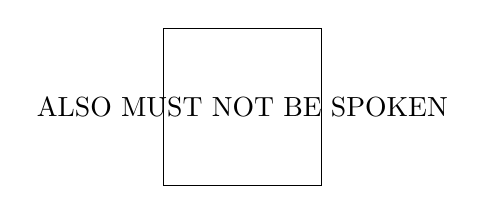
\begin{tikzpicture}
  \draw (0,0) -- (2,0) -- (2,2) -- (0,2) -- cycle;
  \node at (1,1) {ALSO MUST NOT BE SPOKEN};
\end{tikzpicture}
\end{FigureBlock}
\FigureDescription{Horizontal axis a runs 0 to 9; vertical axis b runs 0 to 9.
The four points are (1,2), (3,4), (6,5) and (8,8).}

\end{qunlist}

\end{document}
